\newpage
\title{LEZIONE 10 25/03/2020}\newline
\textbf{link} \href{https://web.microsoftstream.com/video/562a82e0-19cc-4f81-9183-eee77c9c45a4?list=user&userId=faa91214-a6f5-40d7-8875-253fd49b8ce1}{clicca qui} \;\;\textbf{[0:26:39 - fine lezione]}
\section{Raggiungibilità e osservabilità}
\subsection{Raggiungibilità (SD LTI a TC SISO)}
Vogliamo capire sotto quali ipotesi la rappresentazione di stato ($A, b, c, d$) e la funzione di trasferimento ($G(s)$) sono rappresentazioni equivalenti di un sistema. Inoltre affronteremo il problema di studiare la stabilità di un sistema dalla fuznione di trasferimento, tenendo in mente che la funzione di trasferimento può avere delle "parti nascoste".
\subsubsection{Definizioni}
Uno \textbf{stato} $\tilde{x}$ si dice \textbf{raggiungibile} (da zero) se esiste un ingresso $\tilde{u}(t)$ tale che 
\[
    \begin{rcases}
        x(0) &= 0 \\
        u(t) &= \tilde{u}(t) \;\; t \geq 0
    \end{rcases} \longrightarrow x(\tilde{t}) = \tilde{x}  \;\;\;\; \tilde{t}< \infty
\]
Cioè uno stato ($\tilde{x}$) è raggiungibile se esiste un ingresso ($\tilde{u}(t)$) che partendo da zero porta il sistema in quel determinato stato in un tempo finito.\newline
\newline
Un \textbf{sistema} si dice (completamente) \textbf{raggiungibile} se ogni stato è raggiungibile.
\subsubsection{Criterio di raggiungibilità}
Come si determina se un sistema dinamico è o meno raggiungibile?\newline
\newline
Introduciamo il Teorema di Cayley-Hamilton: Ogni matrice annulla il polinomio caratteristico.\newline
Capiamo meglio questo terema guardando il polinomio caratteristico di una matrice $A$ che è il determinante della matrice $sI-A$:
\[
    \Pi(s) = det(sI-A) = s^n + \beta_1 s^{n-1} + \dots + \beta_n
\]
quindi, se calcoliamo il polinomio caratteristico in $A$, vediamo questo si annulla:
\[
    \Pi(A) = det(AI-A) = det(0) = 0
\]
Ne segue che
\[
    A^n + \beta_1 A^{n-1} + \dots + \beta_n I = 0
\]
\[
    A^n = -\beta_1 A^{n-1} - \beta_2 A^{n-2} - \dots - \beta_n I
\]
cioè la potenza ennesima della matrice $A$ può essere scritta come combinazione lineare di tutte le potenze inferiori, fino alla potenza $0$, cioè la matrice identità.\newline
\newline
Applichiamo questo concetto al calcolo del movimento.\newline
Scriviamo la formula di Lagrange nel caso $x(0) = 0$ (cioè solamente movimento forzato):
\[
    x(t) = \int_{0}^{t}e^{A(t-\tau)} b u(\tau) d \tau
\]
dove la matrice $e^{A(t - \tau)}$ è
\[
    e^{A(t - \tau)} = I +A(t-\tau) + \frac{A^2(t-\tau)^2)}{2!} + \dots + \frac{A^{n-1} (t - \tau)^{n-1}}{(n-1)!} +\; \text{[combinazione lineare dei termini precedenti]}\;\dots 
\]
di conseguenza posso fare dei raccoglimenti di tutti i termini "combinazione lineare dei termini precedenti" e scrivere questo termine grazie a una sommatoria:
\[
    e^{A(t - \tau)} = \sum_{l=0}^{n-1} \gamma_l(t-\tau) \cdot  A^l
\]
Ora quindi sostituiamo questo risultato nell'espressione del movimento forzato:
\[
    x(t) = \int_{0}^{t} \sum_{l=0}^{n-1} \gamma_l(t-\tau) \cdot  A^l b u(\tau)d \tau=
\]
dove $\gamma_l(t-\tau)$ sono termini che non mi interessa calcolare, ma mi basta sapere che ci sono e che rappresentano i termini "combinazione lineare dei termini precedenti",
\[
    = \sum_{l=0}^{n-1} A^l b \int_{0}^{t}\gamma_l (t-\tau) u(\tau)d \tau=
\]
chiamiamo ora l'integrale $\zeta_l (t) = \int_{0}^{t}\gamma_l (t-\tau) u(\tau)d \tau$, che dipende solo da $t$ perchè $\tau$ muore durante l'integrazione, inoltre, siccome $\gamma_l$ sono termini di cui non ci interessa la forma, non ci interessa calcolare $\zeta_l (t)$, ci basta sapere che è presente.\newline
\newline
Siamo quindi giunti a scrivere che
\[
    x(t) = \sum_{l=0}^{n-1} A^l b \zeta_l(t)
\]
Il termine $\zeta_l(t)$ contiene
\begin{itemize}
    \item i coefficienti del polinomio caratteristico di $A$;
    \item l'ingresso.
\end{itemize}
\ \newline
Vediamo la scrittura matriciale:
\[
    x(t) = \left[\begin{matrix}
        b & Ab & A^2 b & \dots & A^{n-1}b
    \end{matrix}\right] \cdot  \left[\begin{matrix}
        \zeta_0(t)\\
        \zeta_1(t)\\
        \dots\\
        \zeta_{n-1}](t)
    \end{matrix}\right]
\]
La prima matrice prende il nome di $M_R=$ \textbf{matrice di raggiungibilità} $=\left[\begin{matrix}
    b & Ab & A^2 b & \dots & A^{n-1}b
\end{matrix}\right] $, dove nel caso SISO ogni suo termine è una matrice colonna $n$x$1$, e quindi in totale è una matrice $n$x$n$.\newline
Invece la seconda matrice (quella colonna) la indichiamo come $Z(t) = \left[\begin{matrix}
    \zeta_0(t)\\
    \zeta_1(t)\\
    \dots\\
    \zeta_{n-1}](t)
\end{matrix}\right]$ ed è composta da scalari, quindi in totale è una matrice $n$x$1$. Notiamo che $Z(T)$, essendo composta da tutti i $\zeta_l(t)$ contiene al suo interno i coefficienti del polinomio caratteristico (che sono fissi e conosciamo) e l'ingresso (che è quello che veramente ci interessa nel concetto di raggiungibilità). Quello che è importante da capire è che $Z(t)$ è una riflessione dell'ingresso.\newline
La moltiplicazione di queste due matrici risulta quindi in una matrice $n$x$1$.\newline
Possiamo quindi scrivere 
\[
    x(t) = M_R \cdot Z(t)
\]
\ \newline
Tornando al concetto di raggiungibilità:\newline
Supponiamo ora di voler portare lo stato (da zero) a $\tilde{x}$. Perchè questo sia possibile, deve esistere una certa $\tilde{Z}(t)$ tale che 
\[
    M_R \tilde{Z}(t) = \tilde{x}
\]
Quindi dire che ciò è possibile, per ogni $\tilde{x}$, equivale a dire che $M_R$ non è singolare.\newline
\newline
\textbf{Sistema raggiungibile se e solo se ($\Leftrightarrow$) $M_R$ è non singolare}, dove:
\[
    M_R= \;\text{matrice di raggiungibilità}\; =\left[\begin{matrix}
        b & Ab & A^2 b & \dots & A^{n-1}b
    \end{matrix}\right]
\]
\subsubsection{Esempi}
\textbf{es.} 
\[
    \begin{cases}
        \dot{x}_1 = -x_1 + u\\
        \dot{x}_2 = -x_2 +u
    \end{cases}
\]
Ovviamente se $x(0) = 0$, risulterà $x_1(t) = x_2(t)$ per ogni $u(t)$; nel senso che, data l'espressione di questi due stati, non potrò mai raggiungere lo stato $x = \left[\begin{matrix}
    k\\j
\end{matrix}\right]$ con $k\neq j$, ma posso solo raggiungere gli stati nella forma $\left[\begin{matrix}
    k\\k
\end{matrix}\right]$.\newline
Quindi qualunque stato con $x_1 \neq x_2$ non è raggiungibile. Verifichiamo ora questa affermazione col criterio esposto prima:
\[
    A = \left[\begin{matrix}
        -1 & 0 \\ 0 & -1
    \end{matrix}\right] \;\;\;\;\;\;\;\; b = \left[\begin{matrix}
        1\\1
    \end{matrix}\right] \;\;\;\;\Longrightarrow \;\;\;\;M_R = \left[\begin{matrix}
        b & Ab
    \end{matrix}\right] = \left[\begin{matrix}
        1 &-1 \\1 & -1
    \end{matrix}\right] \;\;\text{singolare}\;
\]
[immagine dagli appunti del prof]
\begin{center}
    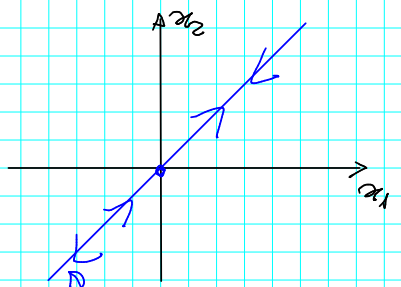
\includegraphics[height=3cm]{../lezione10/img1.PNG}
\end{center}

Esprimiamo lo spazio di stato con un piano di assi $x_1, x_2$, notiamo che lo stato non può muoversi liberamente in tutto lo spazio, ma è vincolata alla retta $x_1 = x_2$ che è il suo sottospazio di raggiungibilità.
\subsection{Osservabilità (SD LTI a TC SISO)}
\subsubsection{Definizioni}
Uno \textbf{stato} $\tilde{x}$ è \textbf{non osservabile} se 
\[
    \begin{rcases}
        x(0) &= \tilde{x}\\
        u(t) &= 0 \;\;\;t \geq 0
    \end{rcases} \longrightarrow y(t) = 0
\]
Cioè uno stato è non osservabile se produce sull'uscita un movimento libero nullo.\newline
\newline
Un \textbf{sistema} è (completamente) \textbf{osservabile} se nessuno stato è non osservabile.
\subsubsection{Criterio di osservabilità}
Chiamiamo $M_O$ una \textbf{matrice di osservabilità} $n$x$n$ definita come:
\[
    M_O = \left[\begin{matrix}
        c' & A'c' & \dots & (A^{n-1})' c'
    \end{matrix}\right]
\]
Abbiamo ottenuto questa matrice con ragionamenti molto simili (che evitiamo di ripetere) a quelli fatti per la matrice di reggiungibilità.\newline
\newline
\textbf{Sistema osservabile se e solo se ($\Leftrightarrow$) $M_O$ è non singolare}.
\subsubsection{Esempi}
\textbf{es.} 
\[
    \begin{cases}
        \dot{x}_1 = -x_1 + u \\
        \dot{x}_2 = 4x_2 +u\\
        y=x_2
    \end{cases}
\]
La relazione tra $u$ e $y$ (cioè fra l'ingresso e l'uscita, la funzione di trasferimento) è tutta racchiusa nelle due ultime righe del sistema, cioè $\dot{x}_1$ non influenza $y$.\newline
Verifichiamo col criterio di osservabilità:\newline
\[
    A= \left[\begin{matrix}
        -1 & 0 \\ 0 & 4
    \end{matrix}\right] = A' \;\;\;\;\;\;\;\; A'c' = \left[\begin{matrix}
        -1 &0 \\ 0 & 4
    \end{matrix}\right] \left[\begin{matrix}
        0 \\ 1
    \end{matrix}\right] = \left[\begin{matrix}
        0 \\ 4
    \end{matrix}\right]
\]
\[
    M_O = \left[\begin{matrix}
        c' & A' c'
    \end{matrix}\right] = \left[\begin{matrix}
        0 & 0 \\ 1 & 4
    \end{matrix}\right] \;\;\text{singolare}\;
\]
\subsection{Osservazioni}
\begin{itemize}
    \item Un sistema può avere parti non raggiungibili e/o non osservabili.\newline
    \newline
    \textbf{es.} Riprendiamo l'esempio fatto precedentemente per la raggiungibilità: \[\begin{cases}
            \dot{x}_1 = -x_1 +u\\
            \dot{x}_2 = -x_2 +u
        \end{cases}
        \] 
        Questo sistema non è completamente raggiungibile, e come si vede a occhio il suo sottospazio di raggiungibilità è la sola retta $x_1 = x_2$. Stato "non raggiungibile" significa che, qualunque sia l'ingresso, non posso raggiungere quel determinato stato a partire da $0$.\newline
        Facciamo un cambio variabili $q_1 = x_1 - x_2$ e $q_2 = x_1 + x_2$ e il sistema diventa: \[
            \begin{cases}
                \dot{q}_1 = \dot{x}_1 - \dot{x}_2 = - x_1 + \cancel{u} + x_2 - \cancel{u} = - q_1\\
                \dot{q}_2 = \dot{x}_1 + \dot{x}_2 = - q_2 + 2 u
            \end{cases} \longrightarrow \begin{cases}
                \dot{q}_1 = -q_1\\
                \dot{q}_2 = -q_2 + 2u
            \end{cases}
        \]
        Con questa trasformazione il significato di "non raggiungibile" cambia: significa che $u$ non influenza una parte dello stato.
        \item Le parti non raggiungibili e/o non osservabili non sono presenti nella funzione di trasferimento: la funzione di trasferimento rappresenta il legame ingresso/uscita e quindi la sola parte raggiungibile e osservabile del sistema.
        \item Gli autovalori delle parti non raggiungibili e/o non osservabili del sistema nel calcolo della funzione di trasferimento sono cancellati (per cancellazione intendiamo il fatto che nel calcolo della funzione di trasferimento alcuni poli e zeri si possno cancellare fra di loro, e questi rappresentano proprio le parti non raggiungibili e/o non osservabili).
\end{itemize}
\ \newline
\textbf{definizione}:  Una calcellazione è \textbf{critica} se avviene al di fuori della regione di asintotica stabilità (a tempo continuo significa che se l'autovalore è cancellato, non ha la parte reale negativa).
\newline
\newline
Conseguenze:
\begin{itemize}
    \item La rappresentazione di stato ($A,b,c,d$) e la funzione di trasferimento ($G(s)$) sono rappresentazioni equivalenti di un sistema dinamico, a meno di una trasformazione di similarità (cioè una trasformazione che preserva gli autovalori), se nel calcolo di $G(s)$ non si hanno cancellazioni o equivalentemente se il sistema è raggiungibile e osservabile.
    \item Poichè i poli di $G(s)$ sono gli autovalori della parte raggiungibile e osservabile del sistema, perchè si possa studiare la stabilità (asintotica) del sistema usando $G(s)$, non vi devono essere cancellazioni critiche.
\end{itemize}
\newpage
\section{Realizzazione}
Per realizzazione si intende partire dalla funzione di trasferimento $G(s)$ e trovare le infinite quaterne $(A,b,c,d)$ corrispondenti: 
\[
    G(s) \rightarrow \infty(A,b,c,d)
\]
Le quaterne $(A,b,c,d)$ costruibili a partire da $G(s)$ sono infinite perchè è sufficiente aggiungere una qualunque "parte nascosta" al nostro sistema per creare una nuova quaterna accettabile.\newline
\newline
Limitandosi al caso in cui la dimensione di $A$ coincide col grado del denominatore di $G(s)$ (cioè realizzando quaterne minime) esistono dei modi "comodi" per trovare una quaterna $(A,b,c,d)$ corrispondente a $G(s)$? Sì.\newline
\newline
Premessa: Se in $G(s)$ il grado del numeratore è uguale al grado del denominatore, allora possiamo esprime $G(s)$ nel seguente modo:
\[
    G(s) = d + \frac{N(s)}{D(s)}
\]
con $d$ costante e grado di $N(s) <$ grado di $D(s)$.\newline
Con questa espressione della funzione di trasferimento, $d$ ce lo abbiamo già e le matrici $A,b,c$ le ricaviamo da $\frac{N(s)}{D(s)}$.\newline
\newline
\textbf{oss.} Questa premessa ci mostra che è sufficiente imparare a trattare il caso in cui $\frac{N(s)}{D(s)}$ ha grado di $N(s) <$ grado di $D(s)$ (perchè avevamo già dimostrato precedentemente che sicurametne $N(s)$ non può avere grado $>$ del grado di $D(s)$, e nel caso in cui il grado di $N(s) = $ grado di $D(s)$ possiamo ricondurci al caso grado di $N(s) <$ grado di $D(s)$).
\subsection{Forma canonica di raggiungibilità}
\subsubsection{Dimostrazione}
Vediamo ora uno dei possibili modi di operare:\newline
Nel caso più estremo il numeratore ha al massimo grado $n-1$:
\[
    G(s) = \frac{ b_1 s^{n-1} + b_2 s^{n-2} + \dots + b_n }{ s^n + a_1 s^{n-1} + \dots + a_n } = \frac{N(s)}{D(s)}
\]
In uno schema a blocchi possiamo quindi rappresentare il blocco della funzione di trasferimento 
\[
    u \rightarrow \left[\frac{N(s)}{D(s)}\right] \rightarrow y
\]
come due blocchi in cascata $\frac{1}{D(s)}$ e $N(s)$
\[
    u \rightarrow \left[\frac{1}{D(s)}\right] \rightarrow \left[N(s)\right] \rightarrow  y
\]
Chiamiamo $X$ il segnale fra i due blocchi $\frac{1}{D(s)}$ e $N(s)$:
\[
    u \rightarrow \left[\frac{1}{D(s)}\right] \rightarrow^X \rightarrow  \left[N(s)\right] \rightarrow  y
\]
\ \newline
Analizzando il primo blocco ($\frac{1}{D(s)}$), ricaviamo le seguenti informazioni sulla struttura della matrice $A$ e $b$:
\[
    \frac{X(s)}{U(s)} = \frac{1}{D(s)} = \frac{1}{ s^n + a_1 s^{n-1} + \dots + a_n }
\]
\[
    X(s) D(s) = U(s)
\]
\[
    s^n X_n + a_1 s^{n-1}X + \dots + a_n X = U
\]
Siccome stiamo operando con funzioni di trasferimento e quindi solo col moto forzato ($x(0) = 0$), allora posso scrivere che $S^n X \;\;\text{diventa}\;\; \frac{d^n x(t)}{dt}$ e quindi:
\[
    \frac{d^n x(t)}{dt^n} + a_1 \frac{d^{n-1} x(t)}{dt^{n-1}} + \dots + a_{n-1} \dot{x}(t) + a_n x(t) = u(t)
\]
Rinominiamo ora i termini nel seguente modo:
\[
    x_n = \frac{d^{n-1} x(t)}{dt^{n-1}}; \;\;\;\;\;\;\;\;\dots; \;\;\;\;\;\;\;\;x_2 = \dot{x}(t); \;\;\;\;\;\;\;\;x_1 = x(t);
\]
e quindi possiamo dire che 
\[
    \begin{cases}
        \dot{x}_1 = x_2;\\
        \dot{x}_2 = x_3;\\
        \dots;\\
        \dot{x}_n = -a_1 x_n - a_2 x_{n-1} - \dots - a_n x_1 + u
    \end{cases}
\]
Quindi vediamo ora le matrici $A$ e $c$ del sistema:
\[
    \left[\begin{matrix}
        \dot{x}_1\\
        \dot{x}_2\\
        \dots\\
        \dot{x}_n
    \end{matrix}\right] = \left[\begin{matrix}
        0 & 1 & 0 & \dots & 0 \\
        0 & 0 & 1 & \dots & 0 \\
        \dots & \dots &\dots&\dots&\dots\\
        0 & 0 & 0 & \dots & 1\\
        -a_n & -a_{n-1} & \dots & \dots & -a_1
    \end{matrix}\right] \left[\begin{matrix}
        x_1\\x_2\\\dots\\x_n
    \end{matrix}\right] + \left[\begin{matrix}
        0\\\dots\\0\\1
    \end{matrix}\right] U
\]
dove la matrice $A$ è composta da una colonna di $0$ accostata a una matrice indentità di dimensione $n-1$ e l'ultima riga è la riga dei coefficienti della funzione di trasferimento; la matrice $b$ è invece composta da un vettore colonna con tutti $0$ tranne l'ultimo elemento che è un $1$.\newline
\newline
Abbiamo quindi fino ad ora trovato $A,b$. Per calcolare $c$ usiamo il secondo blocco ($N(s)$) dello schema a blocchi:
\[
    u \rightarrow \left[\frac{1}{D(s)}\right] \rightarrow^X \rightarrow  \left[N(s)\right] \rightarrow  y
\]
Scriviamo
\[
    Y(s) = N(s) X(s) = (b_1 s^{n-1} + b_2 s^{n-2} + \dots + b_n) X(s)
\]
Dove il termine $b_1 s^{n-1} X(s)$, nel dominio del tempo, diventa $\rightarrow  b_1 \frac{d^{n-1}x(t)}{t^{n-1}} = b_1 x_n(t)$.\newline
Allo stesso modo $b_2 s^{n-1}X(s) \rightarrow b_2 x_{n-1}(t)$.\newline
\dots \newline
E così fino al termine $b_n X(s) \rightarrow  b_n x_1(t)$.\newline
Assemblando il tutto otteniamo la matrice $c$:
\[
    y(t) = \left[\begin{matrix}
        b_n & b_{n-1} & \dots & b_1
    \end{matrix}\right] x(t)
\]
\subsubsection{Metodo pratico}
Presa una funzione di trasferimento, per ottenere una quaterna ($A,b,c,d$) di dimensione minima si procede così: se il grado del numeratore è uguale al grado del denominatore si fa la divisione e si ottiene $G(s) = d + \frac{N(s)}{D(s)}$, da cui si ricava il valore $d$. A questo punto riscriviamo la frazione $\frac{N(s)}{D(s)} = \frac{ b_1 s^{n-1} + b_2 s^{n-2} + \dots + b_n }{ s^n + a_1 s^{n-1} + \dots + a_n }$ e scriviamo le $A, b$ e $c$:
\[
    A=\left[\begin{matrix}
        0 & 1 & 0 & \dots & 0 \\
        0 & 0 & 1 & \dots & 0 \\
        \dots & \dots &\dots&\dots&\dots\\
        0 & 0 & 0 & \dots & 1\\
        -a_n & -a_{n-1} & \dots & \dots & -a_1
    \end{matrix}\right] \;\;\;\;\;\;\;\; b=\left[\begin{matrix}
        0\\\dots\\0\\1
    \end{matrix}\right] \;\;\;\;\;\;\;\; c=\left[\begin{matrix}
        b_n & b_{n-1} & \dots & b_1
    \end{matrix}\right]
\]